% bram_access_topology.tex — ONE source, ONE rendered SVG (bram_access_topology.svg), embedded in
% ../index.md.
%
% The claim: the memory is INSIDE the wrapper and OUTSIDE the kernel.  That boundary is the whole
% reason this example exists — a shared memory has no expression inside a Vitis kernel, so it lives
% beside it as hand-written Verilog and a generated wrapper joins the two.  The nesting is therefore
% the content: two boxes, not one, with `bram_t2p` in the gap between them.
%
% This is the index page's figure, where a rendered SVG reads better than a flowchart.
%
% Render: bash render.sh   (MiKTeX pdflatex -> PDF -> dvisvgm --pdf -> SVG)
\documentclass[tikz,border=4pt]{standalone}
\usepackage{tikz}
\usetikzlibrary{arrows.meta,positioning,calc,fit,backgrounds}

\definecolor{nyuviolet}{HTML}{57068C}
\definecolor{nyuultra}{HTML}{330662}
\definecolor{nyupale}{HTML}{EFE6F5}
\definecolor{nyumid}{HTML}{8A5FB0}
\definecolor{memfill}{HTML}{F1EFF3}
\definecolor{memline}{HTML}{6E6A73}
\definecolor{inkgray}{HTML}{444444}

\begin{document}
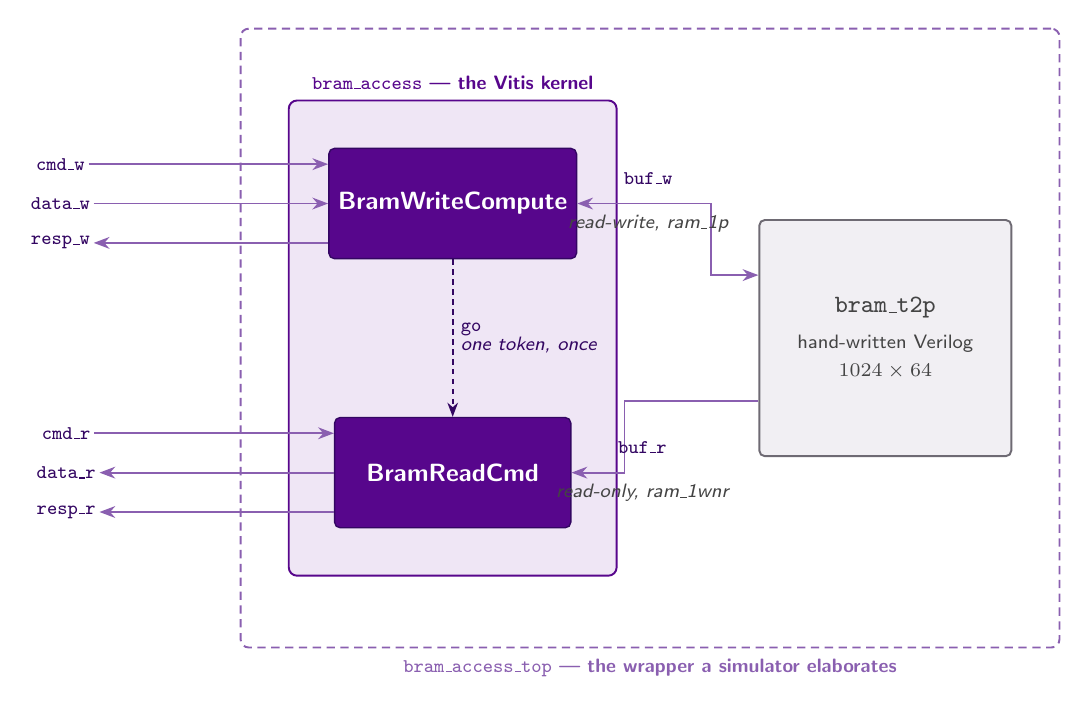
\begin{tikzpicture}[
  font=\sffamily\small,
  task/.style  = {draw=nyuultra, line width=0.5pt, fill=nyuviolet, rounded corners=2pt,
                  minimum width=30mm, minimum height=14mm, text=white, align=center,
                  font=\sffamily\small\bfseries},
  mem/.style   = {draw=memline, line width=0.7pt, fill=memfill, rounded corners=2pt,
                  minimum width=32mm, minimum height=30mm, text=inkgray, align=center},
  kbox/.style  = {draw=nyuviolet, line width=0.7pt, fill=nyupale, rounded corners=3pt},
  wbox/.style  = {draw=nyumid, line width=0.7pt, dash pattern=on 3pt off 2pt, rounded corners=3pt},
  ln/.style    = {-{Stealth[length=2mm]}, draw=nyumid, line width=0.7pt},
  go/.style    = {-{Stealth[length=1.8mm]}, draw=nyuultra, line width=0.6pt,
                  dash pattern=on 2pt off 1.6pt},
  lbl/.style   = {font=\sffamily\scriptsize, text=nyuultra, inner sep=1.2pt},
  sub/.style   = {font=\sffamily\scriptsize\itshape, text=inkgray, inner sep=1.1pt},
  port/.style  = {font=\sffamily\scriptsize\ttfamily, text=nyuultra, inner sep=1.2pt},
]

% --- the two tasks, inside the kernel -------------------------------------------------------------
\node[task] (wr) {BramWriteCompute};
\node[task, below=20mm of wr] (rd) {BramReadCmd};
\draw[go] (wr) -- node[lbl, right=0.5mm, align=left] {\texttt{go}\\[-1pt]\itshape one token, once} (rd);

\begin{scope}[on background layer]
  \node[kbox, fit=(wr)(rd), inner xsep=5mm, inner ysep=6mm] (kernel) {};
\end{scope}
\node[lbl, above=0.8mm of kernel.north, text=nyuviolet, font=\sffamily\scriptsize\bfseries]
  {\texttt{bram\_access} --- the Vitis kernel};

% --- the memory, outside the kernel ---------------------------------------------------------------
\node[mem] (mem) at ([xshift=34mm]kernel.east |- kernel) {\textbf{\texttt{bram\_t2p}}\\[2pt]
  \scriptsize hand-written Verilog\\[-1pt]\scriptsize $1024 \times 64$};

% Elbowed into the memory's own edge rather than to a point beside it.  Labels placed explicitly
% on the horizontal run: `pos=` on a multi-segment path put them back over the task box.
\draw[{Stealth[length=2mm]}-{Stealth[length=2mm]}, draw=nyumid, line width=0.7pt]
  (wr.east) -- ++(17mm,0) |- ([yshift=8mm]mem.west);
\node[port] at ([xshift=9mm, yshift=3.2mm]wr.east) {buf\_w};
\node[sub]  at ([xshift=9mm, yshift=-2.6mm]wr.east) {read-write, ram\_1p};

\draw[ln] ([yshift=-8mm]mem.west) -- ++(-17mm,0) |- (rd.east);
\node[port] at ([xshift=9mm, yshift=3.2mm]rd.east) {buf\_r};
\node[sub]  at ([xshift=9mm, yshift=-2.6mm]rd.east) {read-only, ram\_1wnr};

% --- the wrapper, containing both -----------------------------------------------------------------
\begin{scope}[on background layer]
  \node[wbox, fit=(kernel)(mem), inner xsep=6mm, inner ysep=9mm] (wrap) {};
\end{scope}
\node[lbl, below=0.8mm of wrap.south, text=nyumid, font=\sffamily\scriptsize\bfseries]
  {\texttt{bram\_access\_top} --- the wrapper a simulator elaborates};

% --- the streams: all six on the left, so none crosses the memory or a title ----------------------
% Three per task at +5 / 0 / -5 mm.  Commands and payload point IN, responses point OUT, and both
% live on the same side because the memory owns the right.
\node[port] (cw) at ([xshift=-34mm, yshift=5mm]wr.west)  {cmd\_w};
\node[port] (dw) at ([xshift=-34mm]wr.west)              {data\_w};
\node[port] (rw) at ([xshift=-34mm, yshift=-5mm]wr.west) {resp\_w};
\draw[ln] (cw.east) -- ([yshift=5mm]wr.west);
\draw[ln] (dw.east) -- (wr.west);
\draw[ln] ([yshift=-5mm]wr.west) -- (rw.east);

\node[port] (cr) at ([xshift=-34mm, yshift=5mm]rd.west)  {cmd\_r};
\node[port] (dr) at ([xshift=-34mm]rd.west)              {data\_r};
\node[port] (rr) at ([xshift=-34mm, yshift=-5mm]rd.west) {resp\_r};
\draw[ln] (cr.east) -- ([yshift=5mm]rd.west);
\draw[ln] (rd.west) -- (dr.east);
\draw[ln] ([yshift=-5mm]rd.west) -- (rr.east);

\end{tikzpicture}
\end{document}
